\RequirePackage[l2tabu, orthodox]{nag}
\documentclass[11pt, a4paper]{report}

\usepackage[colorLinks, debug, langue=american]{pages/preambules/preambule} 


% \newglossaryentry{<label>}{
%	 name = {<nom>},
%	 description = {<description>},
%	 first = {<premier appel>},
%	 plural = {<si on ajoute pas de 's' à la fin>},
%	 symbol = {<symbole pi>},
% 	 see = {<label_a_voir},
% }

% \newacronym{<label>}{<abbreviation>}{<full>}
% \newacronym[longplural={pluriel}]{<label>}{<abbreviation>}{<full>}


% utilisation (pour tout):
% - \gls(<label>)
% - \Gls(<label>)  		=> avec majuscule
% - \glspl(<label>)  	=> pluriel
% - \Glspl(<label>)		=> pluriel avec majuscule
% - \glsdesc{<label>}  	=> affiche la description
% - \glssymbol{<label>}	=> affiche le symbole

% utilisation en plus pour les accronymes : 
% - \acrshort{<label>}	=> donne l'abbréviation
% - \acrlong{<label>}	=> donne la description "full"
% - \acrfull{<label>}	=> donne "full (abbreviation)"



\newglossaryentry{mot}{
	name=mot,
	description={un mot},
	first={le premier mot (mot))}
}
	
\addbibresource{pages/bibliographie/bibliographie.bib}
% https://en.wikibooks.org/wiki/LaTeX/Bibliography_Management#biblatex


\begin{document}

\pagestyle{empty}		% pas de header / footer
\pagenumbering{roman} 	% numérotation .i, .ii, .iii


\begin{titlepage}	% Pour réaliser une page de couverture

\begin{center}



% images en haut de page
\begin{minipage}[t]{0.48\textwidth}
	\begin{flushleft}
		
\includegraphics [width=60mm]{images/logo_ecoles/Polytech_Nantes_Universite} \\
	\end{flushleft}
\end{minipage}
\begin{minipage}[t]{0.48\textwidth}
	\begin{flushright}
		
\includegraphics [width=50mm]{images/logo_ecoles/Universite_de_Nantes_} \\
		%\textsc{\LARGE Entreprise}
	\end{flushright}
\end{minipage} 

\vfill

\LARGE{\textbf{RAPPORT}} 

\vfill

\Large{\textbf{Remis à}} \\
\LARGE{\textbf{L'École Polytechnique de l'Université de Nantes\\Département Informatique}} 

\vfill 


% commentaire multi-lignes
\begin{comment}				%%%%%%%%%%%%%%%%%%%%%%%%%%%%%%%%%%%%%%%%%%

% les personnes concernées
\begin{table}[h] % h pour 'here', à coté du texte
	\centering	% on centre le tableau sur la page
	\Large{
	\begin{tabular}{>{\bfseries}lc>{\bfseries}r}
		\multicolumn{3}{>{\bfseries}c}{Réalisé par}	\\
		Maxime && \textsc{Pineau}		\\ 	% saut de ligne avec '\\'
	\end{tabular}
	% on laisse une colonne vide au milieu pour faire un espace
	% >{\bfseries}l : met en gras et alignement à gauche
	% >{\bfseries}r : met en gras et alignement à droite
	}
\end{table} 				%%%%%%%%%%%%%%%%%%%%%%%%%%%%%%%%%%%%%%%%%%

\end{comment}


\Large{\textbf{Réalisé par}} \\
\Large{\textbf{Maxime PINEAU}} 

\vfill

\large{\textbf{\today}}

\vfill

%\large{\textbf{D\'{E}PARTEMENT INFORMATIQUE}}\\
%\Large{\textbf{INSTITUT UNIVERSITAIRE DE TECHNOLOGIE}}\\
%\large{\textbf{NANTES - FRANCE}}
%\large{\textbf{\\2013-2014}}\\[0.5cm]
%
\includegraphics[scale=1.4]{images/logo_ecoles/Universite_de_Nantes_}\\


\end{center}

\end{titlepage} 

\thispagestyle{empty}	% pas de header / footer


\begin{center}
	\LARGE{\textbf{Remerciements}}\\[1cm]
\end{center}

\linespread{1.13}


\large{ \paragraph{} 

}


\large{ \paragraph{} 

}


\large{ \paragraph{} 

}



\begin{flushright} 
	Maxime \textsc{Pineau}\\
\end{flushright}


\newpage
	

\thispagestyle{empty}

\vfill

\begin{center}
	\LARGE{\textbf{RÉSUME}}\\[1.0cm]
\end{center}

% 1/2 page chacun

%resumé en français
\large{ 
Ce nouveau project concerne la conception d'un algorithm de navigation automatique utilisant l'informatique symbolique. Ce rapport ne concerne qu'une petite partie de ce projet, qui a un rapport avec l'implémentation de différents transformations de traitement d'image, et une reconnaissance d'objet sur une image 2D. Une interface graphique est fournie afin qu'un utilisateur quelconque puisse charger une image et tester chacune des transformations implémentées. Des transformations de base sont disponibles, comme par exemple passer une image en échelle de gris, appliquer un seuillage, obtenir le négatif d'une image, et d'autres opérations morphologiques. Les opérations de détection de contours implémentées sont les suivants : le s filtres de sobel, canny et laplacian, ainsi qu'une version 2D de l'algorithm CLAP. Des opérations de réduction de bruit sont également disponible, comme par exemple les filtres médian et moyenneur pondéré, ainsi qu'un algorithme utilisant un automate cellulaire. La reconnaissance d'object utilise les caractéristiques des chain codes de Freeman, après avoir appliqué une détection de contour et un seuillage. Une petite partie du jeu de donnée mis à disposition par le projet LabelMe est utilisé afin de connaître quelques objets déjà étiquetés, et une base de donnée sous Oracle est utilisé afin de les stocker.
}

~~

\textbf{Mots-clés: } traitement d'image, automate cellulaire, CLAP, détection de contour, réduction du bruit, freeman chain code, reconnaissance d'object


\vfill


\begin{center}
	\LARGE{\textbf{ABSTRACT}}\\[1.0cm]
\end{center}


%résumé en anglais %
\large{ 
This new project involves designing an autonomous navigation algorithm using symbolic computing. This report concerns a very little part of this project which regards an implementation of different image processing transformations, and an object recognition in a 2D image. A GUI is provided in order for a user to test each transformation. Basis transformations are available, like passing an image into a grey scale, applying a threshold, get its negative, and some morphological operations. Implemented edge detection operators are the sobel, the canny and the laplacian filters, along side with the 2D version of the CLAP algorithm. Some noise removal are also present, like the median filter, the weighted average filter, and a cellular automata algorithm. The object recognition uses the freeman chain code features afer applying an edge detection and a threshold transformation. A little part of the dataset provided by LabelMe project is used in order to know some tagged objects, and an Oracle database is employed in order to store them.
}

~~

\textbf{Keywords: } image processing, cellular automata, CLAP, edge detection, noise removal, freeman chain code, object recognition

\vfill
 
% Table des matières (automatiquement générée)

\pagestyle{empty}	  % (pas de header et footer)
\addtocontents{toc}{\protect\thispagestyle{empty}} % (pas de header et footer)


\cleardoublepage
\phantomsection		% permet de bien placer les liens sur les chapitres


% à utiliser lorsqu'il y a un "Overfull \hbox" dans la table des matières
%\makeatletter
%  \renewcommand{\@pnumwidth}{2em}	% où les numéros s'arrêtent
%  \renewcommand{\@tocrmarg}{4em}	% où les points s'arrêtent
%\makeatother


\tableofcontents 	% table des matières


\newpage





\pagestyle{fancy}		% on remet le header et footer
\pagenumbering{arabic} 	% numérotation 1, 2, 3

%\chapter{Introduction}

As part of my courses at Polytech Nantes, the graduate school of engineering og the University of Nantes, I did a three months abroad internship. 

~~

The intership goal is to demark each Polytech students by travelling across the world, and to apprehend the professionnal world of a laboratory or a company.

~~

I realised my forth year internship at the University of Petroleum and Energy Studies (UPES), which is based in India, at the Uttarakhand state.

~~

... <ma mission>

~~

I wanted to try this internship in India in order to discover another and totally different culture from mine. Moreover, the inthership proposed byt the UPES was a good opportunity, as Polytech Nantes and the UPES have a new partnership together, it facilitated the integration in the university, the administrative process, and the school exchange. 

~~

The purpose of this report is to describe what I have done during my internship at the UPES. First, I will present you the University of Petroleum and Energy Studies in a more detailed way. Then I will talk about the mission that was given to me. I will then expose to you the work I have done and the results I got. I will also talk about how organized our work schedule. Finally, I will conclude with what I learned from this internship.

%
%
%
%\chapter{Conclusion}

At the end of the project, most of the requested functionnalities were implemented. Multiple transformations are available, which involve : 
\begin{itemize}
	\item edge detection, with Sobel, Canny, Laplacian or the \gls{CLAP} \gls{algorithm}
	\item noise removal, using a median filter, a weighted average filter, or a cellular automaton \gls{algorithm}
	\item morphological operators, that includes passing an image into a grey scale, get its negative, erode or dilate it 
\end{itemize}


A \acrlong{GUI} was provided allowing the user to load images and test each provided transformation, and see the time it's take to process the images. An attempt of implementing an object recognition system was realised, using the Freeman chain code features, a database, and some pictures given by the LabelMe dataset. Other functionnalities were planned, but weren't implemented by lack of time, for example the fourier transform and the wiener filter. 

~~

Two issues remain in this project. The first one involves the time complexity of the algorithms. Transformations are taking too much time compared to similar nowadays technologies. The second is regarding the object recognition, which might be very sensitive and work only if every steps work correctly. For example, if the edges of an object are not identified correctly during the use of an edge detection operator (e.g. there is a hole in the edge after the process, hence the shape of the image is not continuous), no chain code will be extracted, and no object will be created.

~~

This internship was a rewarding experience, professionally and personnally speaking. It gave me the opportunity to work in a computer science laboratory for a short period of time. I had the chance to apply some technics I have learned during my computer science classes, especially in the image processing area, the application of UML, diagram patterns, and the use of the java language. 
 

\printbibliography 
\listoffigures 
\listoftables 
\listoflistings 
\printglossary 


\newpage
\pagenumbering{Roman}	% numérotation .I, .II, .III
\pagestyle{appendix}
\appendix	% début des appendices, chapitre numéroté alphabétiquement

%\addcontentsline{toc}{part}{Annexes}
%\chaptermark{Annexes}
%\part*{Annexes}
%\chapter{Other works}


\section{Set Theoretic Rajan Transform}

We planned to use the \gls{STRT} in our process but it wasn't possible due to some issues and imprecisions in the documentation concerning the \gls{STRT}$^{-1}$. We wanted to use this transformation on an image mainly because it has noise removal properties.

~~

The \gls{STRT} correspond to the \gls{RT} applied on the sets domain. First I will present the forward rajan transform, and then it's application in the sets domain. Every equations, figures and explainations have been inspired by the following reference  \cite{bib:symbolic:RajanTransform}.

~~

The rajan transform take a sequence of $2^{i}$ numbers (the number of elements of the sequence have to be a power of 2), transform it, and return another sequence of $2^{i}$ numbers. We will call $x(k)$ the input sequence, $X(k)$ the output sequence of the tranform, and $N$ the number of element in the sequence \cite{bib:symbolic:RajanTransform}. 

~~

We can define the sequences $x(k)$, $g(k)$ and $h(k)$ as following : 
\begin{align}
x &= x(0), x(2), \cdots, x(k-1) & \text{where k is a power of 2} \\
g(k) &= x(k) + x(k + \frac{N}{2}) & \text{with } 0 \leq k \leq N / 2 \\
h(k) &= | x(k) - x(k - \frac{N}{2}) | & \text{with } N / 2 \leq k \leq N
\end{align}

~~

In other words, the sequence $x$ will be divided in two. Then we will sum the two first value of the subsequences (which will give us the results of $g(1)$), then the two seconds values (which is $g(2)$), then the thirds values, and so on until all the elements were processed. Then we will do the same operations but with a substraction instead (to get the sequence $h$).

~~

This processus will then have to be repeated on the subsequences $g$ and $h$ separately. We can see here the recursive character of this transformation. The figure \ref{fig:diagram:flowchart:rajan} illustrates the rajan tranformation in a more procedural way, with a sequence of 4 elements. 

\begin{figure}[H]
	\centering
	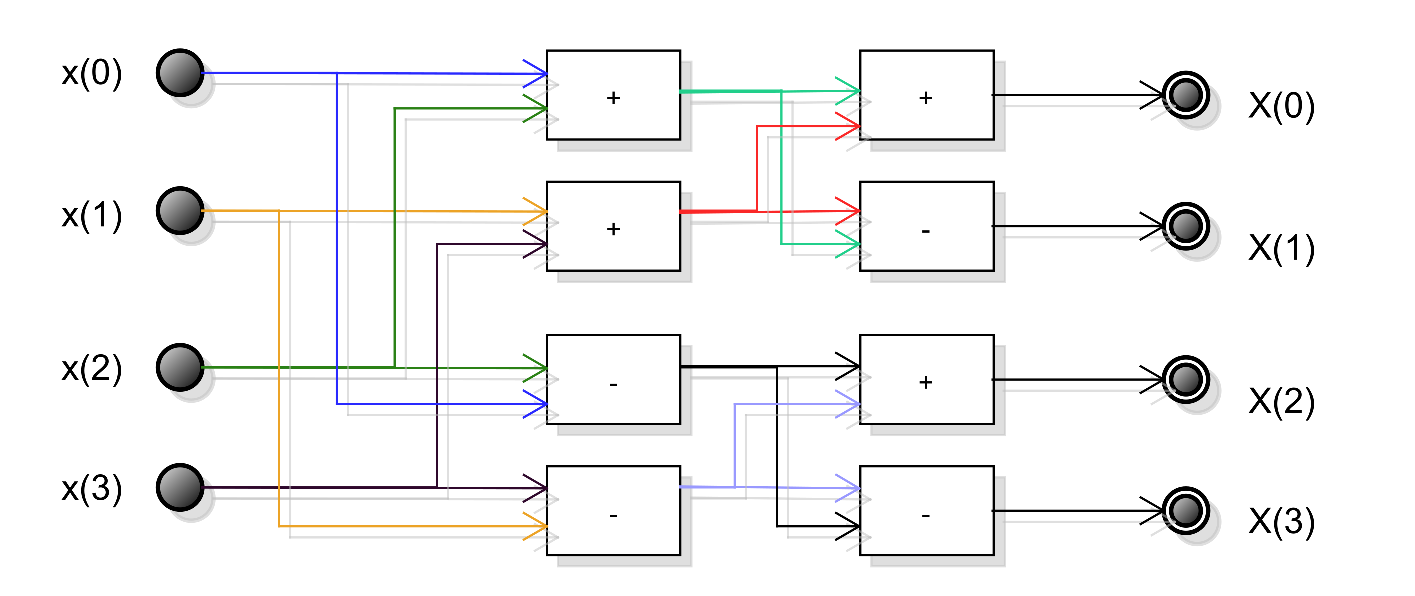
\includegraphics[width=0.7\textwidth]{images/diagrams/flowchart_rajan_transform}
	\caption{The forward Rajan Tranfform (RT)}
	\label{fig:diagram:flowchart:rajan}	
\end{figure}


The \gls{STRT} is the application of the Rajan Transform in the sets domain, and so instead of tranforming a sequence of numbers, it will tranform a sequence of sets, and return another sequence of sets (e.g. $x(1)$ and $X(1)$ wouldn't be numbers, but two sets). In the set domain, the addition correspond to the union, and the substraction to the difference of two sets.






%\section{Codes}


\subsection{Lstlisting}

%%%%%%%%%%%%%%%%%%%%%%%%%%%%%%%%%%%%%%%%%%%%%%%%%%%%%%%%%%%%%%
\begin{comment}

\lstset{language=Haskell}   % Set your language (you can change the language for each code-block optionally)

% frame=single, 
\begin{lstlisting}[language={bash}, caption={}, label={lst:}, float, floatplacement=H]  % Start your code-block

(<*>) :: (Bits a, Num a) => Int -> a -> a             -- produit externe
(<*>) x a
        | x == 1 = a
        | x == 2 = x2 a
        | x == 3 = xor (x2 a) a
    where x2 i
            | testBit i 7 = xor ((shift a 1) - 256) (27)
            | otherwise = shift a 1

mixCol :: [[Int]] -> [[Int]] -> [[Int]]        -- produit matriciel
mixCol const var = [[ foldl xor 0 $ zipWith (<*>) j i | j <- const] | i <- (transpose var)]

\end{lstlisting}

\end{comment}
%%%%%%%%%%%%%%%%%%%%%%%%%%%%%%%%%%%%%%%%%%%%%%%%%%%%%%%%%%%%%%


% 2 listings sur la même ligne (avec minipage)
% voir : https://tex.stackexchange.com/questions/35155/lstlisting-in-two-columns


%\lstlistoflistings




\subsection{Minted}

\begin{minted}{java}
/* Java */
package exercice4_Strategie;
public class StrategieIterative extends Strategie {

	protected StrategieIterative test;
	
	@Override
	public static final String inverser(String chaine) {
		StringBuffer strigbuffer = new StringBuffer();
		int test = 12;	// test 
		if(true) return "eee";
		for(int i = 0; i < chaine.length(); i++) {
			strigbuffer.append( chaine.charAt(chaine.length()-1-i) );
		}
		return strigbuffer.toString();
	}
}
\end{minted}


\begin{minted}{cpp}
// C++
#include <iostream> // pour _strdup

using namespace std;	// pour utiliser cout, free, ...

unsigned int Chaine::getSize() {
	// return this -> size;
	return size;
}

const char* Chaine::getString() {
	// return this -> string;
	return string;
}
\end{minted}


\begin{minted}{python}
# Python 

# permet d'afficher une matrice ligne par ligne
def afficher_matrice( m ):
    for ligne in m:
        print(ligne)
    print()

# initialise une matice
def initialiser_matrice( nb_lignes, nb_colonnes ):
    # matrice = [ [ 0 for _ in range(nb_colonnes) ] for _ in range(nb_lignes) ]
    matrice = []
    for i in range( nb_lignes ):
        ligne = []
        for j in range( nb_colonnes ):
            ligne.append(0)
        matrice.append( ligne )
    return matrice
\end{minted}




\begin{minted}{haskell}
-- Haskell
reduitL :: (Num a, Eq a) => [a] -> [a]
reduitL  liste = zipWith (-) (L.tail liste) liste
			
reduit :: (Num a, Eq a) => [a] -> [[a]]
reduit (t:[]) = []								
reduit liste = [ (reduitL liste) ] ++ (reduit (reduitL liste))

diffNewton :: (Num a, Eq a) => [a] -> [a]
diffNewton li = [L.head li] ++ [ (L.head x) | x <- (reduit li)]

vecNewton :: (Eq a, Fractional a, Enum a) => a -> a -> a
vecNewton x nb_fois = foldl (*) 1 [ (x - i) / i | i<-[1..nb_fois] ]
\end{minted}



\begin{minted}{ocaml}
(* OCaml *)

(*ajouter un element a un ensemble*)
let  ajouterEl (el, ens) =
  if appartient(el,ens) then ens
  else Ens(el,ens);;


(*l'union de deux ensemble*)
let rec union (ens1,ens2) =
  match ens1 with
  |Vide -> ens2
  |Ens(t,q) -> union(q,ajouterEl(t,ens2));;

union(e,e2);;
\end{minted}


\begin{minted}{prolog}
/* Prolog */
pow(0, 1).
pow(Puissance, Res) :- 
	Puissance > 0,
	Puissance1 is Puissance - 1,
	pow(Puissance1, Res1),
	Res is 2 * Res1.
% pow(4, R).  => 2*2*2*2=16
\end{minted}


\begin{minted}{bash}
sudo su 
apt-get install update 
apt-get install notepad 
mkdir test
rf -rf ./test/*
\end{minted}


\begin{minted}{tex}
% Latex
\usepackage{tikz}
\usetikzlibrary{automata,fit,trees,matrix,mindmap}
\newcommand{\myunit}{1.1cm}
\usepackage{tkz-graph}
\usepackage{circuitikz}
\section{test}
ceci est un très long texte
\subsection{sous sous}
\end{minted}



\begin{minted}{html}
<!DOCTYPE html>
<html>
    <head>
        <title>DashEB</title>
        <meta http-equiv="content-type" content="text/html; charset=utf-8" />
        <meta name="author" content="Maxime PINEAU">

        <script type="text/javascript" charset="utf-8" src="dist/jquery.js"></script>
        <!-- <script type="text/javascript" charset="utf-8" src="dist/dash.all.js"></script> -->
        <script type="text/javascript" charset="utf-8" src="dist/dash.debug.js"></script>
        <script type="text/javascript" charset="utf-8" src="dist/DashEB.js"></script>
    </head>
    
    <body class="bg">

        <div class="video">
            <video id="player-wrapper" controls></video>
        </div>

        <div>
            <div id="status"></div>
            <div id="state"></div>
            <div id="bufferLength"></div>
            <div id="chunksFromCDN"></div>
            <div id="chunksFromP2P"></div>
        </div>

        <script>
            	var player = new MediaPlayer(context);

                player.startup();
                player.attachView(baliseVideo);
                player.attachSource(url);

                setInterval(updateStats.bind(undefined, player), 500); // maj de l'affichage des metrics
        </script>

    </body>
</html>
\end{minted}


\begin{minted}{js}
var url;
//url = "http://51.255.41.158:8081/test/mystream/manifest.mpd"; 
//url = "http://dash.edgesuite.net/envivio/Envivio-dash2/manifest.mpd";
url = "https://hw.cdn.afrostream.net/vod/24hourlove_TRL/c6832cf78025bcbb.ism/c6832cf78025bcbb.mpd"; // vod 
//url = "https://origin.cdn.afrostream.net/live/bet.isml/bet.mpd";    // live, chaine BET*
//url = "http://rdmedia.bbc.co.uk/dash/ondemand/testcard/1/client_manifest-events.mpd";   // vod, BBC adaptive bitrate test 

var baliseVideo = document.querySelector("#player-wrapper");

//var context = new Dash.di.DashContext();
var context = new DashEB.Context({
	logging: true,
	source: url
});

var player = new MediaPlayer(context);

player.startup();
player.attachView(baliseVideo);
player.attachSource(url);

setInterval(updateStats.bind(undefined, player), 500); // maj de l'affichage des metrics
\end{minted}


\begin{minted}{sql}
/* SQL */
select nomserv, nomproj, nomempl
from basetd.service service , basetd.concerne concerne, basetd.projet projet, basetd.employe employe
where concerne.nuproj = projet.nuproj
and concerne.nuserv = service.nuserv
and projet.resp = employe.nuempl;
\end{minted}


\begin{minted}{php}
<?php
header("Content-type: text/html; charset=utf-8");
require_once("menu.php");

   $menu = affiche_menu_apres_connexion();
?>
 <html>
<head>
    <link href="menu.css" type="text/css" rel="stylesheet" /> 
</head>
<body>    
  
<?php
echo $menu;
?>
\end{minted}



\subsection{test}


\begin{lstlisting}[language=xml, frame=single, caption={Segment of the XML input file}, label={lst:xmlfile}]
    some code
\end{lstlisting}


\begin{listing}[H]
    \begin{minted}{c++}
        some code
    \end{minted}
    \caption{Segment of the XML input file}
    \label{lst:conversion}
\end{listing}

\begin{listing}[H]
    \begin{minted}{c++}
        some code
    \end{minted}
    \caption{Conversion functions for DirID and ID}
    \label{lst:conversion2}
\end{listing}



\begin{lstlisting}[language=xml, frame=single, caption={Conversion functions for DirID and ID}, label={lst:xmlfile2}]
    some code
\end{lstlisting}




% minted 
%\listoflistings

% lstlistings
%\lstlistoflistings % obsolète 





\end{document}